\usetikzlibrary{angles,quotes,decorations.pathreplacing}
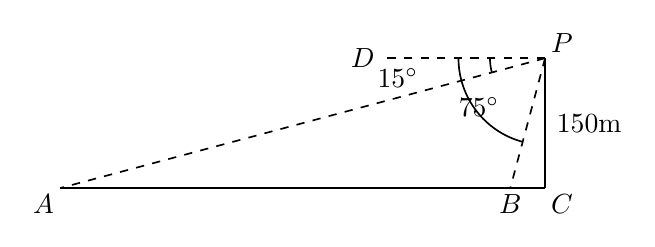
\begin{tikzpicture}[x=1cm,y=1cm,font=\normalsize,
 geometry edge/.style={solid,line width=.6pt},
 geometry mark/.style={solid,line width=.6pt},
 geometry label/.style={font=\normalsize,inner sep=2pt}]
\coordinate (A) at (0.330000000,0.000000000);
\coordinate (B) at (6.047910000,0.000000000);
\coordinate (C) at (6.490000000,0.000000000);
\coordinate (P) at (6.490000000,1.650000000);
\coordinate (D) at (4.400000000,1.650000000);
\coordinate (L15) at (4.620000000,1.400000000);
\coordinate (L75) at (5.650000000,1.030000000);
\coordinate (LM) at (7.050000000,0.825000000);
\draw[geometry edge] (A)--(B);
\draw[geometry edge] (B)--(C);
\draw[geometry edge] (P)--(C);
\draw[geometry edge,dashed] (P)--(A);
\draw[geometry edge,dashed] (P)--(B);
\draw[geometry edge,dashed] (P)--(D);
\pic[draw, geometry mark, angle radius=7mm] {angle=D--P--A};
\pic[draw, geometry mark, angle radius=11mm] {angle=D--P--B};
\node[geometry label,below left] at (A) {$A$};
\node[geometry label,below] at (B) {$B$};
\node[geometry label,below right] at (C) {$C$};
\node[geometry label,above right] at (P) {$P$};
\node[geometry label,left] at (D) {$D$};
\node[geometry label] at (L15) {$15^\circ$};
\node[geometry label] at (L75) {$75^\circ$};
\node[geometry label] at (LM) {$150\mathrm{m}$};
\end{tikzpicture}
